\section{Mathemathik-Hilfen}

\subsection{Trigonometrie}

% Copy-Paste from KomFour

\begingroup
\renewcommand{\arraystretch}{2}
\setlength{\tabcolsep}{0mm}
\scalebox{0.33}{
\Huge
\begin{tabularx}{3\columnwidth}{rp{1mm}V{3}*{17}{C}}
    \rowcolor{subsectioncolor!30}$\bm{\alpha}$\phantom{${}^{\circ}$} && $0$ & $\dfrac{\pi}{6\mathstrut}$ & $\dfrac{\pi}{4}$ & $\dfrac{\pi}{3}$ & $\dfrac{\pi}{2}$ & $\dfrac{2\pi}{3}$ & $\dfrac{3\pi}{4}$ & $\dfrac{5\pi}{6}$ & $\pi$ & $\dfrac{7\pi}{6}$ & $\dfrac{5\pi}{4}$ & $\dfrac{4\pi}{3}$ & $\dfrac{3\pi}{2}$ & $\dfrac{5\pi}{3}$ & $\dfrac{7\pi}{4}$ & $\dfrac{11\pi}{6}$ & $2\pi$ \\\hline
    \rowcolor{subsectioncolor!30}$\bm{\alpha^\circ}$ && \phantom{${}^\circ$}$0^\circ$ & $30^\circ$ & $45^\circ$ & $60^\circ$ & $90^\circ$ & $120^\circ$ & $135^\circ$ & $150^\circ$ & $180^\circ$ & $210^\circ$ & $225^\circ$ & $240^\circ$ & $270^\circ$ & $300^\circ$ & $315^\circ$ & $330^\circ$ & $360^\circ$ \\\hline
    $\bm{\sin(\alpha)}$ && $0$ & $\dfrac{1}{2\mathstrut}$ & $\dfrac{\sqrt{2}}{2}$ & $\dfrac{\sqrt{3}}{2}$ & $1$ & $\dfrac{\sqrt{3}}{2}$ & $\dfrac{\sqrt{2}}{2}$ & $\dfrac{1}{2}$ & $0$ & $-\dfrac{1}{2}$ & $-\dfrac{\sqrt{2}}{2}$ & $-\dfrac{\sqrt{3}}{2}$ & $-1$ & $-\dfrac{\sqrt{3}}{2}$ & $-\dfrac{\sqrt{2}}{2}$ & $-\dfrac{1}{2}$ & $0$ \\\hline
    $\bm{\cos(\alpha)}$ && $1$ & $\dfrac{\sqrt{3}}{2\mathstrut}$ & $\dfrac{\sqrt{2}}{2}$ & $\dfrac{1}{2}$ & $0$ & $-\dfrac{1}{2}$ & $-\dfrac{\sqrt{2}}{2}$ & $-\dfrac{\sqrt{3}}{2}$ & $-1$ & $-\dfrac{\sqrt{3}}{2}$ & $-\dfrac{\sqrt{2}}{2}$ & $-\dfrac{1}{2}$ & $0$ & $\dfrac{1}{2}$ & $\dfrac{\sqrt{2}}{2}$ & $\dfrac{\sqrt{3}}{2}$ & $1$ \\\hline
    $\bm{\tan(\alpha)}$ && $0$ & $\dfrac{\sqrt{3}}{3\mathstrut}$ & $1$ & $\sqrt{3}$ & $\pm\infty$ & $-\sqrt{3}$ & $-1$ & $-\dfrac{\sqrt{3}}{3}$ & $0$ & $\dfrac{\sqrt{3}}{3}$ & $1$ & $\sqrt{3}$ & $\pm\infty$ & $-\sqrt{3}$ & $-1$ & $-\dfrac{\sqrt{3}}{3}$ & $0$ \\\hline
    $\bm{\cot(\alpha)}$ && $\pm\infty$ & $\sqrt{3}$ & $1$ & $\dfrac{\sqrt{3}}{3\mathstrut}$ & $0$ & $-\dfrac{\sqrt{3}}{3}$ & $-1$ & $-\sqrt{3}$ & $\pm\infty$ & $\sqrt{3}$ & $1$ & $\dfrac{\sqrt{3}}{3}$ & $0$ & $-\dfrac{\sqrt{3}}{3}$ & $-1$ & $-\sqrt{3}$ & $\pm\infty$ \\
\end{tabularx}}
\endgroup


\subsection{Lineare Algebra -- Repetition}

Der Anhang B des Skripts (S. 279 ff.) beschreibt die Matrizenrechnung. Hier werden nur einige Ausschnitte erwähnt.


\subsubsection{Matrixmultiplikation}

Die Spaltenzahl von $\bm{A}$ muss mit der Zeilenzahl von $\bm{B}$ übereinstimmen! \\
Dimensionen: $\bm{A} \in \mathbb{C}^{m \times n}, \, \bm{B} \in \mathbb{C}^{n \times p} \quad \Rightarrow\ \bm{C} \in \mathbb{C}^{m \times p}$


\example{Matrixmultiplikation}
% Beispiel von LinAlg
$A =
	\begin{pmatrix}
		\crd{1} & \crd{2}   & \crd{4}   \\
		0       & 4         & -1
	\end{pmatrix}$, \qquad 
$B =
	\begin{pmatrix}
		\cbl{-2}    & 4     \\
		\cbl{-4}    & -5    \\
		\cbl{2}     & 4
	\end{pmatrix}$
	
\smallskip

$C = A \cdot B =
	\begin{pmatrix}
		\crd{1} \cdot ({\cbl{-2}}) + {\crd{2}} \cdot ({\cbl{-4}}) + \crd{4} \cdot \cbl{2}   &
		\crd{1} \cdot 4 + \crd{2} \cdot (-5) + \crd{4} \cdot 4                              \\
		0 \cdot ({\cbl{-2}}) + 4 \cdot (\cbl{-4}) + (-1) \cdot \cbl{2}                      &
		0 \cdot 4 + 4 \cdot (-5) + (-1) \cdot 4
	\end{pmatrix}
    = 
    \begin{pmatrix}
		-2  & 10    \\
        -18 & -24
	\end{pmatrix}$


\subsubsection{Übersicht zu (quadratischen) Matritzen}

Die Aussagen innerhalb einer Spalte sind jeweils äquivalent.

\begin{ctabular}{l c l}
    \toprule
    $A \in \mathbb{C}^{n \times n}$ ist regulär         & & $A \in \mathbb{C}^{n \times n}$ ist singulär            \\
    \midrule
    $\det(A) \neq 0$                                    & & $\det(A) = 0$                                           \\
    \midrule
    Die Inverse $A^{-1}$ existiert                      & & Die Inverse $A^{-1}$ existiert \textbf{nicht}           \\
    \midrule
    $n$ Spaltenvektoren von $A$                         & & $n$ Spaltenvektoren von $A$ sind                        \\
    sind linear unabhängig                              & & \textbf{nicht} linear unabhängig                        \\
    \midrule
    $n$ Zeilenvektoren von $A$                          & & $n$ Zeilenvektoren von $A$                              \\
    sind linear unabhängig                              & & sind \textbf{nicht} linear unabhängig                   \\
    \midrule
    $A$ hat vollen Rang:                                & & $A$ hat \textbf{nicht} vollen Rang:                     \\
    $\mathrm{rang}(A) = n$                              & & $\mathrm{rang}(A) < n$                                  \\
    \bottomrule
\end{ctabular}

\textrightarrow\ Die oberen drei Zeilen gelten \textbf{nur für quadratische Matritzen}


\subsubsection{Determinante}

Die Determinante ist nur für \textbf{quadratische} Matritzden definiert

\smallskip

\begin{minipage}[c]{0.38\columnwidth}
    \begin{itemize}
        \item $A = \begin{bmatrix} 
                        a_{11} 
                    \end{bmatrix} 
                    \quad \Rightarrow \det(A) = a_{11}$
    \end{itemize}
\end{minipage}
\hfill
\begin{minipage}[c]{0.6\columnwidth}
    \begin{itemize}
        \item $A = \begin{bmatrix}
                        a_{11}  & a_{12}    \\
                        a_{21}  & a_{22}
                    \end{bmatrix}
                    \quad \Rightarrow \det(A) = a_{11} a_{22} - a_{12} a_{21}$ 
    \end{itemize}
\end{minipage}


\begin{minipage}[c]{0.38\columnwidth}
    \begin{itemize}
        \item $A = \begin{bmatrix}
                        a_{11}  & a_{12}    & a_{13}    \\
                        a_{21}  & a_{22}    & a_{23}    \\
                        a_{31}  & a_{32}    & a_{33}    
                    \end{bmatrix}$
    \end{itemize}
\end{minipage}
\hfill
\begin{minipage}[c]{0.6\columnwidth}
    \begin{align*}
        \Rightarrow \det(A) &= a_{11} a_{22} a_{33} + a_{12} a_{23} a_{31} + a_{13} a_{21} a_{32}\\
                            &- a_{11} a_{23} a_{32} - a_{12} a_{21} a_{33} - a_{13} a_{22} a_{31}
    \end{align*}
\end{minipage}

\smallskip

\begin{itemize}
    \item Bei einer Diagonalmatrix oder einer Dreieicksmatrix entspricht die Determinante dem Produkt der Diagonalelemente
\end{itemize}


\subsubsection{Singuläre / Reguläre Matritzen}

\begin{itemize}
    \item Eine Matrix $A \in \mathbb{C}^{n \times n}$ ist singulär, falls $\det(A) = 0$
    \item Eine Matrix $A \in \mathbb{C}^{n \times n}$ ist regulär, falls $\det(A) \neq 0$
\end{itemize}


\subsubsection{Rang einer Matrix}

\begin{itemize}
    \item Der Rang einer Matrix $A \in \mathbb{C}^{m \times n}$ bestimmt sich als Anzahl linear unabhängiger Spaltenvektoren
        (was zugleich der Anzahl linear unabhängiger Zeilenvektoren ist)
    \item Der Maximal mögliche Rang ist $\min(m, \,n)$
\end{itemize}



\subsubsection{Inverse Matritzen}

Eine Matrix ist invertierbar, wenn sie regulär ist.

\smallskip

\begin{minipage}[c]{0.38\columnwidth}
    $A = \begin{bmatrix} 
            a_{11} 
        \end{bmatrix} 
        \quad \Rightarrow A^{-1} = \frac{1}{a_{11}}$
\end{minipage}
\hfill
\begin{minipage}[c]{0.6\columnwidth}
    $A = \begin{bmatrix}
            a_{11}  & a_{12}    \\
            a_{21}  & a_{22}
        \end{bmatrix}
        \quad \Rightarrow A^{-1} = \frac{1}{\det(A)} \begin{bmatrix}
                                        a_{22}      & - a_{12}    \\
                                        - a_{21}    & a_{11}
                                        \end{bmatrix}$
\end{minipage}

\smallskip

\begin{itemize}
    \item Für $n \geq 3$ empfiehlt sich der Gauss-Jordan Algorithmus
    \item Die Inverse von Diagonalmatritzen kann durch Inversion der Diagonalelemente berechnet werden
\end{itemize}
%------------------ neu ------------------
\subsubsection{Permutationsmatrix}

Eine Permutationsmatrix $P \in \mathbb{R}^{n \times n}$ entsteht durch Vertauschen von
Zeilen der Einheitsmatrix. Es gilt:
\[
P^{-1} = P^T, \qquad P^T P = I
\]

Eine Rotation um den Winkel $\alpha$ wird beschrieben durch:
\[
R(\alpha) =
\begin{pmatrix}
\cos\alpha & -\sin\alpha \\
\sin\alpha & \cos\alpha
\end{pmatrix}
\]
Eigenwerte:
\[
\lambda_{1,2} = e^{\pm j\alpha}
\]
Reell nur für $\alpha = k\pi$.
%-----------------------------------------------

\subsubsection{Lineare Gleichungssysteme lösen}

\vspace{-0.2cm}

$$ \bm{A} \cdot \vec{x} = \vec{b} \quad \Leftrightarrow \quad \vec{x} = \bm{A^{-1}} \cdot \vec{b} $$
%----------------------- neu ------------------
Ein lineares Gleichungssystem $A x = b$ besitzt genau dann eine eindeutige Lösung, wenn
\[
\det(A) \neq 0 \quad \Leftrightarrow \quad \mathrm{rang}(A) = n
\]
In diesem Fall gilt:
\[
x = A^{-1} b
\]
%-----------------------------------------------
\subsubsection{Transformationen}

\begin{minipage}[c]{0.7\columnwidth}
    \raggedright
    Die Transformationsmatrix $\bm{T}$ kann eine Drehung, Rotation, Projektion oder Permutation von $\vec{p}$ verursachen. \\
    Permutation: Reihenfolge ändern (\textrightarrow\ Permutationsmatritzen haben nur eine 1 pro Zeile und Spalte und sind orthagonal)
\end{minipage}
\hfill
\begin{minipage}[c]{0.25\columnwidth}
    $$ \vec{q} = \bm{T} \cdot \vec{p} $$
\end{minipage}



\subsubsection{Eigenwerte / Eigenvektoren}

Um die Eigenwerte $\lambda_i$ einer (quadratischen) Matrix $\bm{A}$ zu berechnen, muss die folgende Gleichung erfüllt sein:
$$ \det(\lambda \cdot \bm{I} - \bm{A}) \overset{!}{=} 0 $$
Die Lösungen dieser charakteristischen Gleichung entsprechen den Eigenwerten $\lambda_i$.

\smallskip

Die Eigenvektoren berechnen sich durch Einsetzen von $\lambda_i$ in die Gleichung(en)
$$ (\lambda_i \bm{I} - \bm{A}) \cdot \vec{v}_i = \vec{0} $$
\textrightarrow\ Eine Koordinate muss gewählt werden, die andere Koordinate ist linear abhängig!

\medskip


\para{Eigenschaften von Eigenwerten und Eigenvektoren}

\begin{outline}
    \1 Bei einer Diagonalmatrix / Dreiecksmatrix entsprechen die Diagonalelemente $a_{ii}$ den Eigenwerten
    \1 Eine singuläre Matrix hat mindestens einen Eigenwert bei Null
    \1 Zwei Eigenwerte $\lambda_i \neq \lambda_j$ haben unabhängig Eigenvektoren $\vec{v}_i$ und $\vec{v}_j$
    \1 Die Eigenwerte von $\bm{A}$ und $\bm{A^{\tps}}$ sind identisch
    \1 Reelle Eigenwerte haben reelle Eigenvektoren
\end{outline}
%----------------------- neu ------------------
\para{Geometrische Interpretation von Eigenvektoren}
Für $A v = \lambda v$ gilt:
\begin{itemize}
\item $|\lambda| > 1$: Streckung
\item $|\lambda| < 1$: Stauchung
\item $\lambda < 0$: Spiegelung
\end{itemize}

\para{Typische Zustandswahl}

Translation:

\[
    x=
    \begin{bmatrix}
        s\\
        \dot s
    \end{bmatrix}
\]

Rotation:

\[
    x=
    \begin{bmatrix}
        \varphi\\
        \dot\varphi
    \end{bmatrix}
\]
%-----------------------------------------------

\subsubsection{Positive Definitheit von Matritzen}

Die Definitheit einer Matrix kann auf mehrere Arten überprüft werden.
Eine Matrix $\bm{Q}$ ist positiv definit ($\bm{Q} > 0$), wenn

\smallskip

\begin{minipage}[t]{0.48\columnwidth}
    \begin{outline}
        \1 \textbf{Alle} Eigenwerte der Matrix grösser Null sind \textrightarrow\ $\lambda_i > 0$
        \1 \textbf{Alle} führenden Hauptminoren positiv sind
            \2 Alle Determinanten der gezeigten 'Untermatritzen' müssen $> 0$ sein
    \end{outline}
\end{minipage}
\hfill
\begin{minipage}[t]{0.48\columnwidth}
    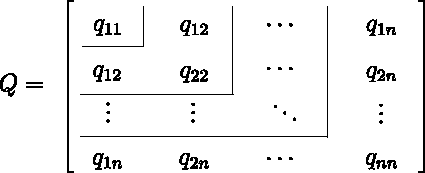
\includegraphics[width=\columnwidth, align=t]{images/hauptminoren.pdf}
\end{minipage}
%==========================================================================================================
\subsubsection{Lagrange-Verfahren}

\[
L=T-V
\]

\[
\frac{d}{dt}
\left(
\frac{\partial L}{\partial \dot q_i}
\right)
-
\frac{\partial L}{\partial q_i}
=
Q_i
\]

Ohne äussere Kräfte gilt:

\[
Q_i=0
\]

\vspace{0.1cm}

\textbf{Vorgehen:}

\begin{enumerate}
    \item $T$ bestimmen
    \item $V$ bestimmen
    \item $L=T-V$
    \item Lagrange-Gleichung anwenden
    \item DGL $\rightarrow$ ZRD $\rightarrow$ Linearisierung
\end{enumerate}
%===============================================================================

\subsubsection{Exponentialfunktion von Matritzen}
\label{Exponentialfunktion von Matritzen}

Die Exponentialfunktion von Matritzen berechnet sich aus der Definition der Taylor-Reihe.

$$ e^{\bm{A} t} = \bm{I} + \bm{A} t + \frac{\bm{A}^2}{2!} t^2 + \cdots + \frac{\bm{A}^k}{k!} t^k + \cdots 
    = \sum\limits_{k=0}^{\infty} \frac{\bm{A}^k t^k}{k!} $$


\paragraph{Spezialfall: Diagonalmatrix}

\vspace{-0.2cm}

$$
\bm{A} = 
\begin{bmatrix}
    a_{11}  & 0         & \cdots    & 0         \\
    0       & \ddots    & \ddots    & \vdots    \\
    \vdots  & \ddots    & \ddots    & 0         \\
    0       & \cdots    & 0         & a_{nn}
\end{bmatrix}
\quad \Rightarrow \quad
e^{\bm{A} t} =
\begin{bmatrix}
    e^{a_{11} \cdot t}  & 0         & \cdots    & 0                 \\
    0                   & \ddots    & \ddots    & \vdots            \\
    \vdots              & \ddots    & \ddots    & 0                 \\
    0                   & \cdots    & 0         & e^{a_{nn} \cdot t}
\end{bmatrix}
$$
%----------------------- neu ------------------
\subsubsection{MATLAB-Hinweis}
\[
A * B \text{ (Matrixmultiplikation)}, \qquad
A .* B \text{ (elementweise Multiplikation)}
\]
%-----------------------------------------------

\subsection[Dezibel \deci \bel]{Dezibel $\boldsymbol{\deci \bel$}}

\vspace{-0.2cm}

$$ \boxed{ |K|_{\deci \bel} = 20 \, \deci \bel \cdot \log_{10} |K| \quad \Leftrightarrow \quad 
            |K| = 10 ^{\big( \frac{|K|_{\deci \bel}}{20 \, \deci \bel}\big)}  } $$

\textbf{Hinweis:} Die Betragsstrichte nur Notation! $|K|$ kann sehr wohl negativ sein!


\subsubsection{Rechenregeln}

\begin{itemize}
    \item Multiplikation \textrightarrow\ Addition 
        \vspace{-0.2cm}
        $$ | K_1 \cdot K_2 |_{\deci \bel} = | K_1 |_{\deci \bel} + | K_2 |_{\deci \bel} $$
    \item Division \textrightarrow\ Subtraktion 
        $$ \Big| \frac{K_1}{K_2} \Big|_{\deci \bel} = | K_1 |_{\deci \bel} - | K_2 |_{\deci \bel} $$
    \item Kehrwert \textrightarrow\ Negatives Vorzeichen 
        $$ \Big| \frac{1}{K_1} \Big|_{\deci \bel} = | 1 |_{\deci \bel} - | K_1 |_{\deci \bel} = - | K_1 |_{\deci \bel} $$
\end{itemize}


\subsubsection[\deci \bel--Umrechnungstabelle]{$\boldsymbol{\deci \bel}$--Umrechnungstabelle}{133}

\begin{minipage}[c]{0.48\columnwidth}
    \begin{ctabular}{c c}
        \toprule
        \textbf{Faktor $\boldsymbol{[1]}$}  & \textbf{Dezibel $\boldsymbol{\deci \bel}$} \\
        \midrule
        $100$                   & $40$  \\ 
        $10$                    & $20$  \\
        $1$                     & $0$   \\
        $0.1$                   & $-20$ \\
        $0.01$                  & $-40$ \\
        \bottomrule
    \end{ctabular}
\end{minipage}
\hfill
\begin{minipage}[c]{0.48\columnwidth}
    \begin{ctabular}{c c}
        \toprule
        \textbf{Faktor $\boldsymbol{[1]}$}  & \textbf{Dezibel $\boldsymbol{\deci \bel}$} \\
        \midrule
        $2$                     & $6$   \\
        $\sqrt{2}$              & $3$   \\
        $\frac{1}{\sqrt{2}}$    & $-3$  \\
        $\frac{1}{2}$           & $-6$  \\
        \bottomrule
    \end{ctabular}
\end{minipage}


\subsection{Spezielle Ansätze PBZ}

\vspace{-0.2cm}

\renewcommand{\arraystretch}{2}
\begin{tabular}{ll}
    $f(x)$  & $ = \frac{5x^2-37x+54}{x^3-6x^2+9x} = \frac{A}{x}+\frac{B}{x-3}+\frac{C}{(x-3)^2} = \frac{A(x-3)^2+Bx(x-3)+Cx}{x(x-3)^2}$ \\ 
    $f(x)$  & $ = \frac{1.5x}{x^3-6x^2+12x-8} = \frac{A}{x-2}+\frac{B}{(x-2)^2}+\frac{C}{(x-2)^3 } =\frac{A(x-2)^2+B(x-2)+C}{(x-2)^3}$  \\
    $f(x)$  & $ = \frac{x^2-1}{x^3+2x^2-2x-12} = \frac{A}{x-2}+\frac{Bx+C}{x^2+4x+6} = \frac{A(x^2+4x+6)+(Bx+C)(x-2)}{(x-2)(x^2+4x+6)}$ \\
\end{tabular}
\renewcommand{\arraystretch}{1}


%\columnbreak

\subsection{Laplace-Transformation}
\label{Laplace-Transformation}


\subsubsection{Laplace-Transformierte einiger Funktionen}{21}
\label{Laplace-Transformierte einger Funktionen}

Alle Funktionen $f(t)$ sind implizit mit dem Einheitssprung $\varepsilon(t)$ multipliziert, sodass die Funktionen nur
für $t \geq 0$ definiert sind.

\vspace{0.2cm}

\begin{minipage}[t]{0.48\columnwidth}
    \begin{center}
        \renewcommand{\arraystretch}{1.4}
        \begin{tabular}{c c c}
            \toprule
            $\bm{f(t)}$                             & $\laplace$    & $\bm{F(s)}$                   \\
            \midrule
            $\delta(t)$                             & $\laplace$    & $1$                           \\
            \midrule
            $\delta(t - T_t)$                       & $\laplace$    & $e^{-T_t s}$                  \\
            \midrule
            $\varepsilon(t)$                        & $\laplace$    & $\frac{1}{s}$                 \\
            \midrule
            $t$                                     & $\laplace$    & $\frac{1}{s^2}$               \\
            \midrule            
            $t^2$                                   & $\laplace$    & $\frac{2}{s^3}$               \\
            \midrule
            $t^n$                                   & $\laplace$    & $\frac{n!}{s^{n+1}}$          \\
            \midrule   
            $e^{at}$                                & $\laplace$    & $\frac{1}{s-a}$               \\  
            \midrule
            $t \cdot e^{at}$                        & $\laplace$    & $\frac{1}{(s-a)^2}$           \\
            \bottomrule
        \end{tabular}
        \renewcommand{\arraystretch}{1}
    \end{center}
\end{minipage}
\hfill
\begin{minipage}[t]{0.48\columnwidth}
    \begin{center}
        \renewcommand{\arraystretch}{1.4}
        \begin{tabular}{c c c}
            \toprule
            $\bm{f(t)}$                             & $\laplace$    & $\bm{F(s)}$                   \\
            \midrule
            $t^n \cdot e^{at}$                      & $\laplace$    & $\frac{n!}{(s-a)^{n+1}}$      \\
            \midrule
            $\sin(bt)$                              & $\laplace$    & $\frac{b}{s^2 + b^2}$         \\
            \midrule
            $\cos(bt)$                              & $\laplace$    & $\frac{s}{s^2 + b^2}$         \\          
            \midrule
            $1 - e^{at}$                            & $\laplace$    & $\frac{-a}{s (s-a)}$          \\
            \midrule
            $e^{at} \cdot \cos(bt)$                 & $\laplace$    & $\frac{s-a}{(s-a)^2 + b^2}$   \\
            \midrule
            $e^{at} \cdot \sin(bt)$                 & $\laplace$    & $\frac{b}{(s-a)^2 + b^2}$     \\
            \midrule
            $\frac{e^{at} - e^{bt}}{a-b}$           & $\laplace$    & $\frac{1}{(s-a)(s-b)}$        \\
            \midrule
            $\frac{a \, e^{at} - b \, e^{bt}}{a-b}$ & $\laplace$    & $\frac{s}{(s-a)(s-b)}$        \\
            \bottomrule
        \end{tabular}
        \renewcommand{\arraystretch}{1}
    \end{center}
\end{minipage}

\vspace{0.2cm}

\textbf{Hinweis:} Der Einheitssprung $\varepsilon(t)$ äussert sich als eine $1$ in der Gleichung im Zeitbereich \\
\textbf{Hinweis:} Teilweise braucht es Umformungen, damit die Tabelle angewendet werden kann


\subsubsection{Eigenschaften der Laplace-Transformation}{22}

\resizebox{\columnwidth}{!}{
    \begin{tabular}{ccc}
        \toprule
        \textbf{Zeitbereich}                                                        & \textbf{Bildbereich}                          & \textbf{Operation im Zeitbereich}     \\
        \midrule
        $a_1 f_1(t) + a_2 f_2(t)$                                                   & $a_1 F_1(s) + a_2 F_2(s)$                     & Superposition                         \\
        \midrule
        $\dot{f}(t)$                                                                & $s F(s) - f(0)$                               & Differentiation ...                   \\
        \midrule
        $\ddot{f}(t)$                                                               & $s^2 F(s) - s f(0) - \dot{f}(0)$              & ...mehrfach angewendet                \\
        \midrule
        $\int_{0}^{t} f(\tau) \, \diff \tau$                                        & $\frac{1}{s} F(s)$                            & Integration                           \\
        \midrule
        $f(t - T_t) \quad [T_t \text{ reell, } \geq 0]$                             & $F(s) \cdot e^{- T_t \, s}$                   & Rechtsverschiebung                    \\
        \midrule
        $f_1(t) * f_2(t) = \int_{0}^{t} f_1(\tau) \cdot f_2(t - \tau) \, \diff t$   & $F_1(s) \cdot F_2(s)$                         & Faltung                               \\
        \midrule
        $f(a \cdot t) \quad [a \text{ reell, } > 0]$                                & $\frac{1}{a} \cdot F \Big( \frac{s}{a} \Big)$ & Skalierung                            \\
        \midrule
        $e^{\mp at} \cdot f(t)$                                                     & $F(s \pm a)$                                  & Dämpfung                              \\
        \bottomrule
    \end{tabular}
}

\subsubsection{Grenzwertsätze der Laplace-Transformation}{22}

\textbf{Achtung:} Grenzwertsätze dürfen nur angewendet werden, wenn Grenzwerte existieren!

\smallskip

\begin{itemize}
    \item Das Anfangswerttheorem gilt für Regelungstechniker immer
    \item Das Endwerttheorem gilt \textbf{nur}, wenn \textbf{System stabil} ist \\
        (Polstellen in linker Halbebene bzw. $\sigma < 0$)
\end{itemize}

\begin{center}
    \begin{tabular}{l c ll}
        \toprule
        \textbf{Zeitbereich}                &       & \textbf{Bildbereich}                          & \textbf{Bezeichnung}      \\
        \midrule
        $\lim\limits_{t \to 0} f(t)$        & $=$   & $\lim\limits_{s \to \infty} s \cdot F(s)$     & Anfangswerttheorem        \\
        \midrule
        $\lim\limits_{t \to \infty} f(t)$   & $=$   & $\lim\limits_{s \to 0} s \cdot F(s)$          & Endwerttheorem            \\
        \bottomrule
    \end{tabular}
\end{center}



\section{Wurzelortskurven (WOK)}
\label{Wurzelortskurven (WOK)}

% WOK aus RegT3
\subsection{Grundsätzliches Aussehen der WOK}

\begin{outline}
    \1 Char. Polynom $N_f(s) = N(s) + K \cdot Z(s)$ hat für jeden $K$-Wert $n$ Wurzeln (Nullstellen)
        \2 Visualisiert: $n$ kontinuierliche Linien (Äste)
    \1 WOK ist immer \textbf{symmetrisch} bezüglich der \textbf{reellen Achse}
    \1 Für $K = 0$ sind die $n$ Wurzeln von $N_f(s)$ und $N(s)$ identisch und entsprechen den $n$ Polen von $G(s)$
    \1 Anfangspunkte der Äste: $n$ Wurzeln von $N(s)$ \textrightarrow\ Kreuze
    \1 Endpunkte der Äste: $m$ Wurzeln von $Z(s)$ \textrightarrow\ Kreise \\
        $n-m$ Äste laufen ins Unendliche
\end{outline}


\subsection{Zeichnen von Wurzelortskurven}{96-98}
\label{Zeichnen von Wurzelortskurven}

\para{1. Pol- / Nullstellenplan}

Pole / Nullstellen von $G(s)$ werden in komplexer Zahlenebene eingetragen:

\vspace{0.1cm}

\begin{outline}
    \1 Pole $p_k$ ($k=1 \ldots n$) werden als $\times$ dargestellt \textrightarrow\ Startpunkte der $n$ Äste
    \1 Nullstellen $z_k$ ($k=1 \ldots m$) werden als $\circ$ dargestellt \textrightarrow\ Endpunkte von $m$ Ästen
\end{outline}

\medskip


\para{2. Reelle Achse}

\begin{enumerate}
    \item Start 'ganz rechts' (weiter rechts als alle Einträge $\times$ bzw. $\circ$) auf reeller Achse starten; Stift 'nicht schreibend' bzw 'oben'
    \item Nach links wandern und bei \textbf{jedem} $\times$ bzw. $\circ$ Stift toggeln \\
        ('nicht schreibend' \textlrarrow\ 'schreibend') \\
        \textrightarrow\ Doppel-Pole bzw. Doppel-Nullstellen entsprechend einem Punkt ('Doppel-Toggel')
\end{enumerate}

\begin{center}
    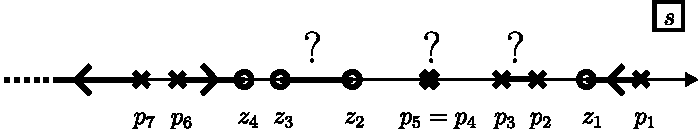
\includegraphics[width=0.78\columnwidth]{images/WOK_zeichnen_reelle_achse.pdf}
\end{center}

\textbf{ \textrightarrow\ Gültige WOK-Äste verbinden einen Pol mit einer Nullstelle.} \\
An den Stellen mit ? (Verbindung von Pol zu Pol bzw. NS zu NS) ist die Situation noch unbefriedigend, da $n > m$. \textrightarrow\ siehe 3. und 4. 

\medskip


\para{3. Asymptoten: Schnittpunkte und Richtungen}

Wenn $n > m$ gilt, dann streben $n-m$ Äste (\textbf{Geraden}) der WOK asymptotisch gegen Unendlich. Zu berechnen ist der \textbf{Schnittpunkt} und 
die \textbf{Richtung der ersten der Asymptoten}. Die weiteren Asymptoten sind dann \textbf{gleichmässig} versetzt.

\smallskip

\begin{minipage}{0.7\columnwidth}
    $$ \text{Schnittpunkt:} \quad \sigma_A = \frac{\sum_{k=1}^{n} \Re{p_k} - \sum_{k=1}^{m} \Re{z_k}}{n-m} $$
\end{minipage}
\hfill
\begin{minipage}{0.28\columnwidth}
    \begin{tabular}{@{}ll@{}}
        $n$ & \# Pole   \\
        $m$ & \# NS 
    \end{tabular}
\end{minipage}

\vspace{0.1cm}

$$ \text{Richtung 1. Asymptote} \quad \phi = \frac{\pi}{n-m} \qquad 
    \text{gleichmässig versetzt um} \quad \frac{2 \pi}{n-m} $$

\begin{center}
    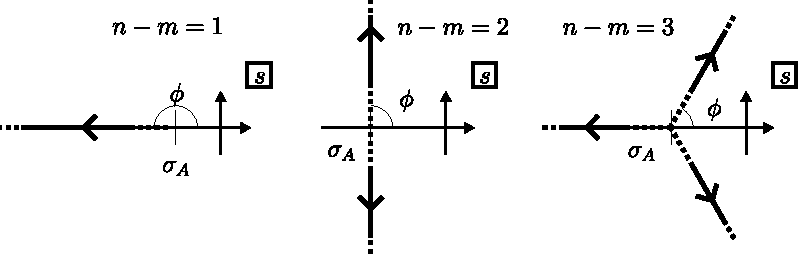
\includegraphics[width=0.8\columnwidth]{images/WOK_asymptoten.pdf}
\end{center}

\vspace{-0.2cm}

\textrightarrow\ Wenn $n-m$ ungerade, dann geht immer eine Asymptote auf reeller Achse nach links

\medskip


\para{4. Verzweigungspunkte / Vereinigungspunkte}

Bei Verbindung von Pol zu Pol bzw. NS zu NS treten Verzweigungen / Vereinigungen auf. In diesen Punkten gilt Folgendes:

\vspace{0.1cm}

\begin{outline}
    \1 Äste treten (meist) \textbf{rechtwinklig aus der reellen Achse} aus.
    \1 Verzweigungspunkt bzw. Vereinigungspunkt befindet sich \textbf{in der Mitte} des Pol- bzw. NS-Paares
    \1 Die \textbf{Form} der betreffenden Äste kann auf zwei Arten verlaufen:
        \2 Kreisförmig in Richtung \textbf{Asymptoten}, welche in der Nähe sind
        \2 Kreisförmig zum nächsten Verzweigungspunkt bzw. Vereinigungspunkt
\end{outline}

\begin{center}
    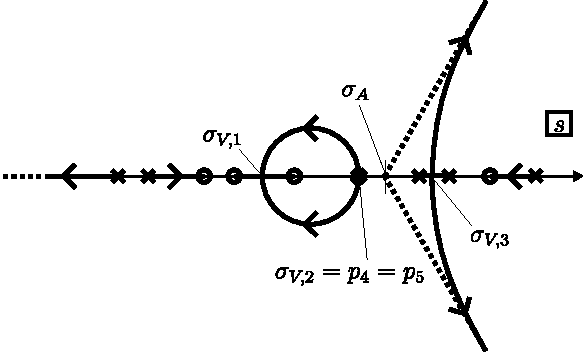
\includegraphics[width=0.7\columnwidth]{images/WOK_komplett.pdf}
\end{center}

\vspace{-0.2cm}

\begin{minipage}[c]{0.58\columnwidth}
    Die genauen Verzweigungspunkte / Vereinigungspunkte können auch mittels folgender impliziter Formel berechnet werden:
\end{minipage}
\hfill
\begin{minipage}[c]{0.4\columnwidth}
    $$ \underbrace{ \sum\limits_{k=1}^{n} \frac{1}{\sigma_V - p_k} }_{\text{Pole}} =
        \underbrace{ \sum\limits_{k=1}^{m} \frac{1}{\sigma_V - z_k} }_{\text{Nullstellen}} $$
\end{minipage}

\vspace{0.1cm}

\textbf{Achtung:} Die Formel kann unbrauchbare Lösungen (z.B. mit $\Im{\sigma_{V,i}} \neq 0$) liefern, welche 'aussortiert' werden müssen.


\subsection{WOK zu einigen geläufigen Pol- / NS-Verteilungen}{99}

\begin{center}
    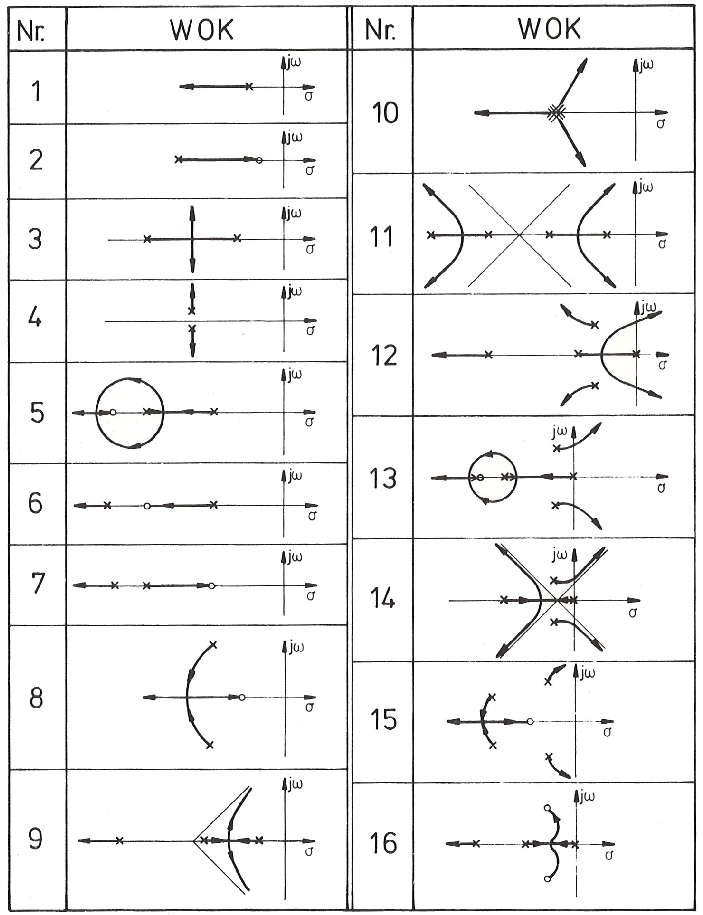
\includegraphics[width=0.9\columnwidth]{images/WOK_pol_NS_tabelle.pdf}
\end{center}



\subsection{Auslegen eines staischen P-Reglers mittels WOK}{{101-102}}

\subsubsection{Vorgehen -- P-Regler mit WOK auslegen}
\label{Vorgehen -- P-Regler mit WOK auslegen}

\begin{enumerate}
    \item WOK skizzieren (inkl. Dämpfung) gemäss Abschnitt \ref{Zeichnen von Wurzelortskurven}
    \item Pole, welche bei variablem $K$ auf Asymptoten wandern so platzieren, dass gewünschte \textbf{Dämpfung} erreicht ist
    \item \textbf{Bandbreite} $\bm{\omega_n}$ und \textbf{Verstärkung} $\bm{K}$ bestimmen, indem einer der in 2. platzierten Pole betrachtet wird \\
        Dabei werden von einem solchen Pol aus \textbf{Verbindungslinien} zu allen weiteren Polen ($\theta_i$) und allen Nullstellen ($\lambda_i$) gezeichnet.
        Die Verstäkung $K$ berechnet sich dann aus den entsprechenden \textbf{Abständen} $\theta_i$ und $\lambda_i$ gemäss
        $$ \boxed{ K = \frac{\prod_{i=1}^{n} \theta_i}{\prod_{i=1}^{m} \lambda_i} = \frac{\theta_1 \cdot \theta_2 \cdot \ldots \cdot \theta_n}{\lambda_1 \cdot \lambda_2 \cdot \ldots \cdot \lambda_m} } $$
        \textrightarrow\ Falls keine Nullstellen vorhanden sind, ist das entsprechende Produkt $=1$
    \item Weitere Verstärkungen (z.B. $K_R$) aus $K$ bestimmen
\end{enumerate}


\example{Auslegung eines P-Regler mittels WOK}

Eine (stabile) Strecke $G_S(s)$ soll mit einem P-Regler mit $G_R(s) = K_R$ mit \textbf{möglichst grosser 
Verstärkung} $\bm{K_R}$ geregelt werden, wobei alle Pole eine \textbf{minimale Dämpfung} $\bm{\zeta = 0.7}$ haben sollen.

\vspace{0.1cm}

Der offene Regelkreis $G_0(s)$ wird betrachtet als

\vspace{-0.1cm}

$$ G_0(s) = K_R \cdot \underbrace{ \frac{5}{s^2 + 6s + 8} }_{G_S(s)} 
    = \underbrace{K_R \cdot 5}_{K} \cdot \underbrace{ \frac{1}{s^2 + 6s + 8}}_{G_S(s)}  $$

Gemäss Abschnitt \ref{Vorgehen -- P-Regler mit WOK auslegen} kann nun der Regler ausgelegt werden und somit $K_R$ aus $K$ bestimmt werden.

\vspace{0.1cm}

\begin{minipage}[t]{0.3\columnwidth}
    \begin{center}
        \myul{\textbf{1. WOK skizzieren}}
    \end{center}

    \vspace{-0.2cm}

    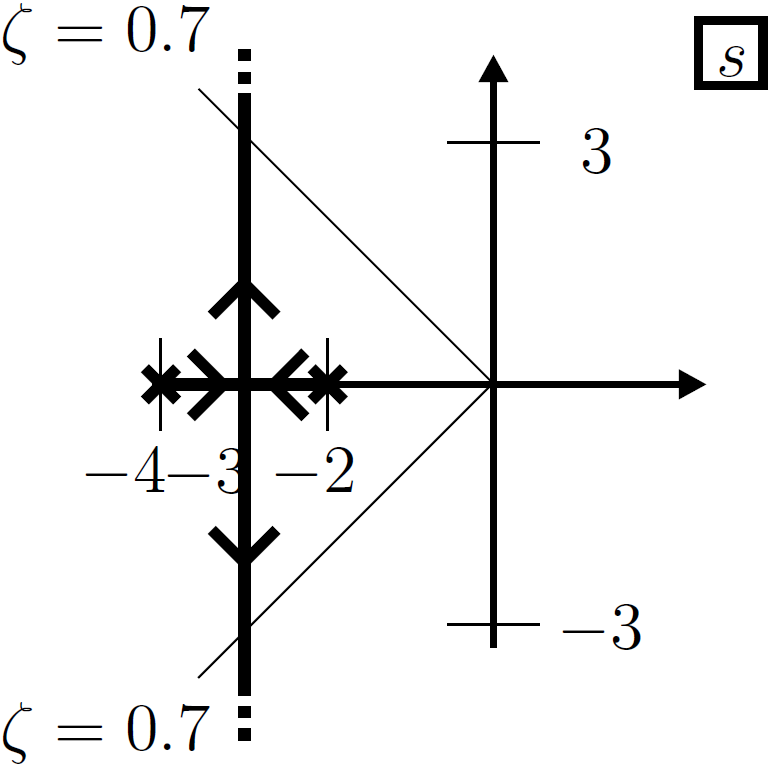
\includegraphics[width=\columnwidth, align=t]{images/WOK_P-Regler_WOK_zeichnen.png}
\end{minipage}
\hfill
\begin{minipage}[t]{0.3\columnwidth}
    \begin{center}
        \myul{\textbf{2. Pole platzieren}}
    \end{center}

    \vspace{-0.2cm}

    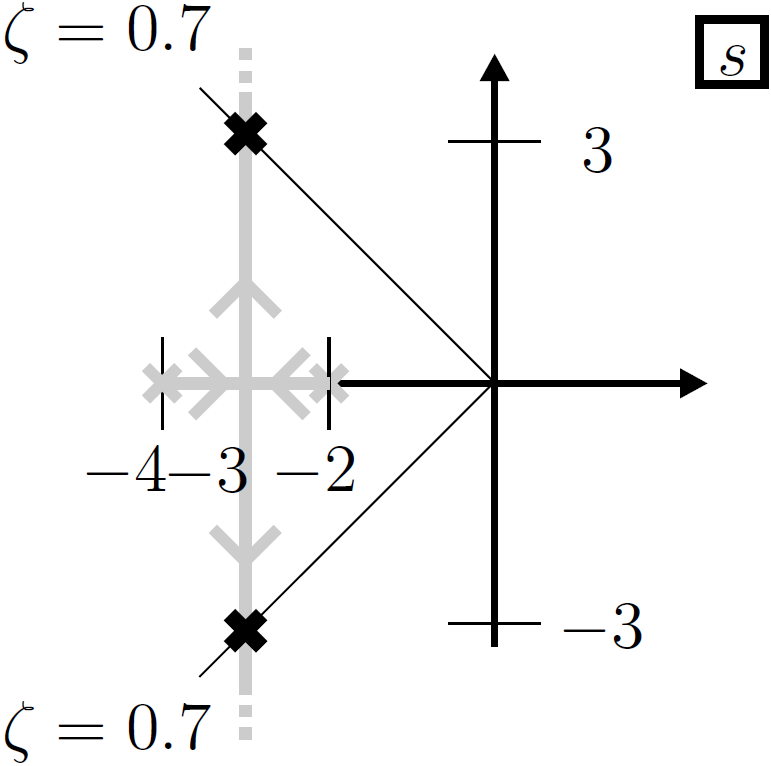
\includegraphics[width=\columnwidth, align=t]{images/WOK_P-Regler_daempfung.png}
\end{minipage}
\hfill
\begin{minipage}[t]{0.3\columnwidth}
    \begin{center}
        \myul{\textbf{3. $\bm{K}$ und $\bm{\omega_n}$ bestimmen}}
    \end{center}
    
    \vspace{-0.2cm}

    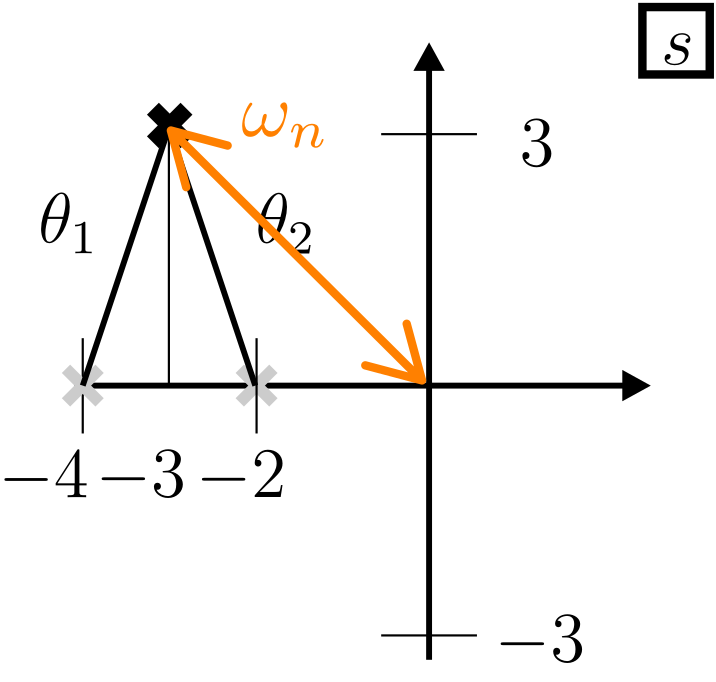
\includegraphics[width=\columnwidth, align=t]{images/WOK_P-Regler_verstaerkung.png}
\end{minipage}

\vspace{0.1cm}

\myul{\textbf{4. $\bm{K_R}$ bestimmen}}

Aus $K = \theta_1 \cdot \theta_2 = \sqrt{1^2 + 3^2} \cdot \sqrt{1^2 + 3^2} = 10$ und $K = 5 \cdot K_R$ ergibt sich $K_R = 5$


\subsubsection{Beantwortung der 'Grundfragen' für P-Regler}

\begin{itemize}
    \item Regelkreis ist stabil, wenn $K$ gross genug gewählt wird, dass alle Pole in RHE sind
    \item Bandbreite: $\omega_n$ aus WOK abgelesen: $\omega_n = \sqrt{3^2 + 3^2} = \sqrt{2 \cdot + 3^2} = \sqrt{2} \cdot 3 \, \frac{\radian}{\second}$
    \item Gewünschte Dämpfung $\zeta = 0.7$ ist einstellbar (Pole konnten so platziert werden)
    \item Stationärer Fehler: $e_{\infty} = \frac{E(s)}{R(s)} = \frac{1}{1 + G_0} \Big|_{s = 0} =\frac{4}{9}$
\end{itemize}


%\columnbreak

\section{Matlab}

\subsection{Zustandsraumdarstellung (ZRD)}

\subsubsection{Zustandsraum-Objekte (LTI-Objekte)}

\lstinputlisting[aboveskip=1mm, belowskip=0mm]{snippets/LTI-Objekte.m}


\subsubsection{Spezielle Matritzen im Zustandsraum}

\lstinputlisting[aboveskip=1mm, belowskip=0mm]{snippets/spezielle_matritzen_zustandsraum.m}


\subsection{Bode- und Nyquist}

\lstinputlisting[aboveskip=1mm, belowskip=0mm]{snippets/bode_nyquist.m}


\subsection{z-Transformation}

\lstinputlisting[aboveskip=1mm, belowskip=0mm]{snippets/z_transformation.m}


\subsection{Implementation eines diskreten Reglers}

\lstinputlisting[aboveskip=1mm, belowskip=0mm]{snippets/digitale_regler.m}


\subsection{Wurzelortskurven}

\lstinputlisting[aboveskip=1mm, belowskip=0mm]{snippets/wurzelortskurven.m}


\subsection{Zustandsrückführungen / Beobachter}

\lstinputlisting[aboveskip=1mm, belowskip=0mm]{snippets/zustandsrueckfuehrung.m}




\section{Statische Grundglieder (ohne Gedächtnis)}

Der Ausgang des Systems ist \textbf{nur} vom aktuellen Eingang abhängig 
$$ y(t) = f( u(t) ) $$
\textbf{Hinweis:} $u(t)$ entspricht meist $A \cdot \varepsilon(t)$ (skalierter Einheitssprung)


\subsection{P-Glied (Proportional)}

\vspace{-0.2cm}

$$ \boxed{ y(t) = K \cdot u(t) } $$

\begin{minipage}{0.23\columnwidth}
    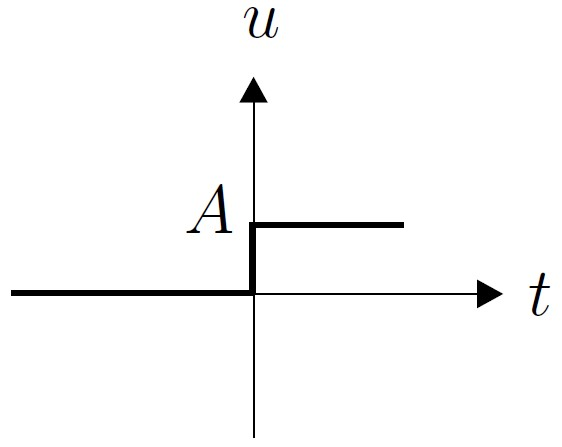
\includegraphics[width=0.8\columnwidth]{images/RegT1_grundglieder/eingangssignal_schrittantwort} 
\end{minipage}
\hfill
\begin{minipage}{0.23\columnwidth}
    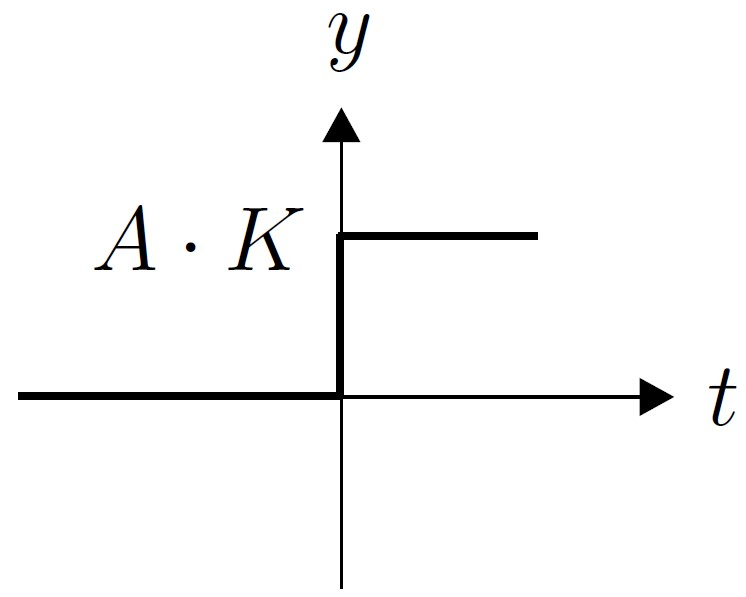
\includegraphics[width=0.8\columnwidth]{images/RegT1_grundglieder/schrittantwort_p-glied} 
\end{minipage}
\hfill
\begin{minipage}{0.23\columnwidth}
    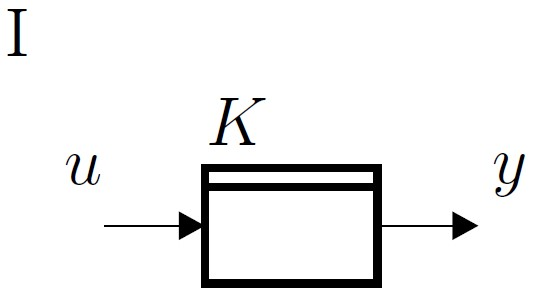
\includegraphics[width=0.8\columnwidth]{images/RegT1_grundglieder/symbol_p-glied_1}
\end{minipage}
\hfill
\begin{minipage}{0.23\columnwidth}
    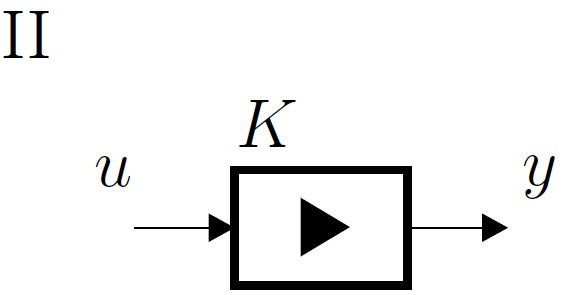
\includegraphics[width=0.8\columnwidth]{images/RegT1_grundglieder/symbol_p-glied_2}
\end{minipage}


\section{Dynamische Grundglieder (mit Gedächtnis)}

Der Ausgang des Systems ist vom aktuellen \textbf{und} von vergangenen Eingängen abhängig.
Vergangene Eingänge werden im System in einem Speicher, einem Zustand $x(t)$ abgelegt. 
$$ y(t) = f( u(t), \, x(t) ) $$


\subsubsection{Prozesse mit / ohne Ausgleich}

\begin{tabular}{ll}
ohne Ausgleich:     & Sprungantwort wächst grenzenlos an \\
mit Ausgleich:      & Sprungantwort strebt gegen endlichen Wert \\
				    & \textrightarrow\ \textbf{Gegenkopplung} am Ausgang
\end{tabular}


\subsection{Totzeit-Glied}

\vspace{-0.2cm}

$$ \boxed{ y(t) =  u(t - T_t) }  $$

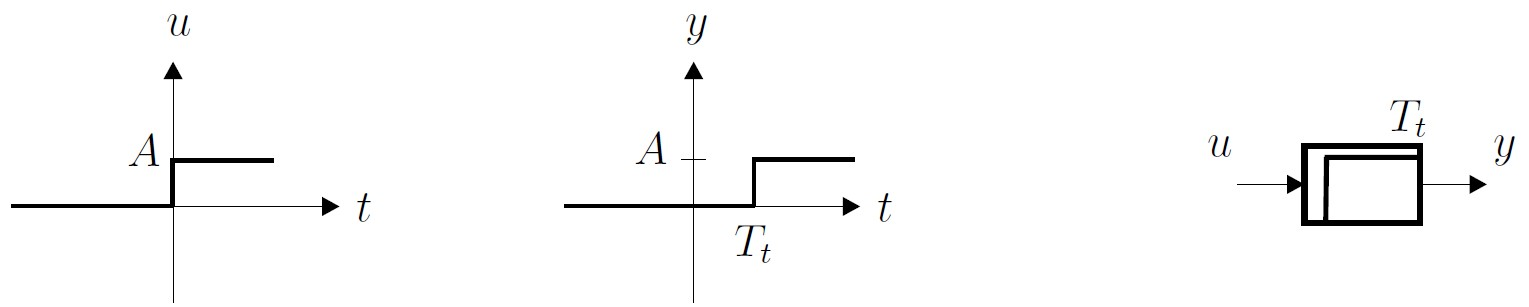
\includegraphics[width=0.9\columnwidth]{images/RegT1_grundglieder/totzeit-glied}


\subsection{I-Glied (Integrierer)}

\begin{minipage}{0.48\columnwidth}
    $$ \boxed{ \text{DGL: } \dot{y}(t) = K \cdot u(t) }  $$
\end{minipage}
\hfill
\begin{minipage}{0.48\columnwidth}
    $$ \boxed{ \scriptstyle{ y = \int\limits_{- \infty}^t u(\tau) \, \diff \tau = K \int\limits_{- \infty}^t u(\tau) \, \diff \tau + y(0) } }$$
\end{minipage}

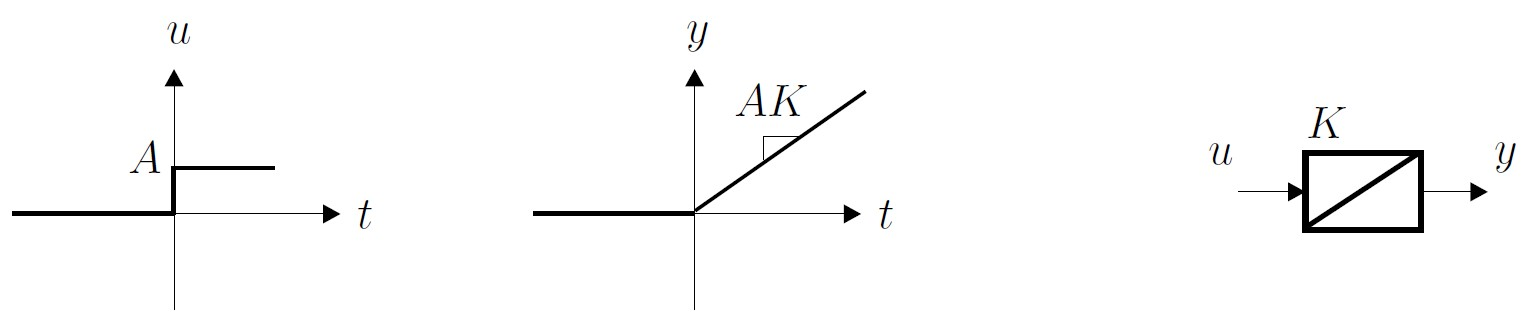
\includegraphics[width=0.9\columnwidth]{images/RegT1_grundglieder/i-glied} 


\subsection[PT1-Glied]{$\text{PT}_1$-Glied}

Ein Energiespeicher \textrightarrow\ System schwingt nicht

\begin{minipage}{0.48\columnwidth}
    $$ \boxed{ \text{DGL: } T \, \dot{y}(t) + y(t) = K \cdot u(t) }  $$
\end{minipage}
\hfill
\begin{minipage}{0.48\columnwidth}
    $$ \boxed{ y(t) = K \, A + (y_0 - K \, A) \cdot e^{- \frac{t}{T}} } $$
\end{minipage}


\begin{minipage}{0.5\columnwidth}
    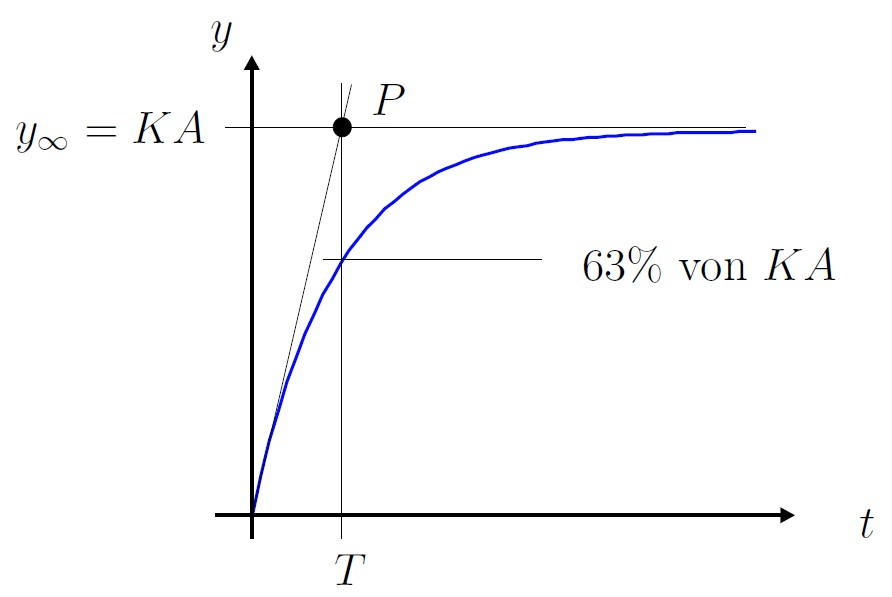
\includegraphics[width=\columnwidth]{images/RegT1_grundglieder/pt1-glied_kennlinie}
\end{minipage}
\hfill
\begin{minipage}{0.4\columnwidth}
    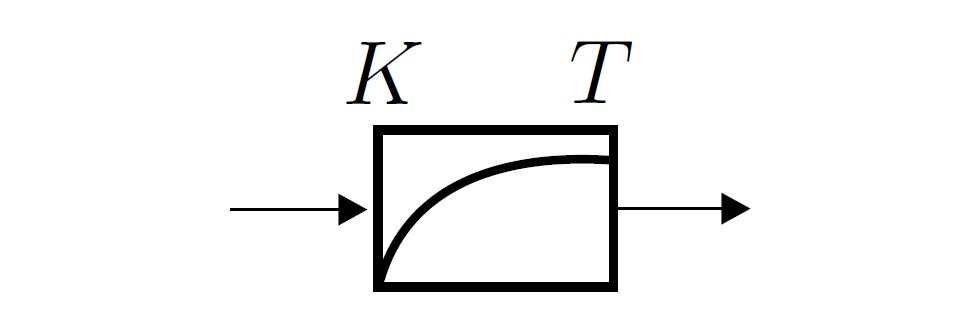
\includegraphics[width=0.8\columnwidth]{images/RegT1_grundglieder/symbol_PT1-glied}
\end{minipage}


\subsubsection{Modellierung einer $\text{PT}_1$ Regelstrecke}

\begin{itemize}
    \item Ausmessen der Sprungantwort $u(t) = A \cdot \varepsilon(t)$ \\
        \textrightarrow\ Die Sprungantwort entspricht dem Diagramm
    \item Parameter $K$ berechnen: $K = \frac{y_\infty}{A}$ 
    \item Parameter $T$ bestimmen: Tangente am Anfang durch Punkt $P$ \\
        oder: Zeit bis $y(T) = 0.63 \cdot K \, A$ erreicht ist \textrightarrow\ $T$ ablesen
\end{itemize}


\example{$\text{PT}_1$-Glied als Blockschaltbild}

\begin{minipage}{0.48\columnwidth}
    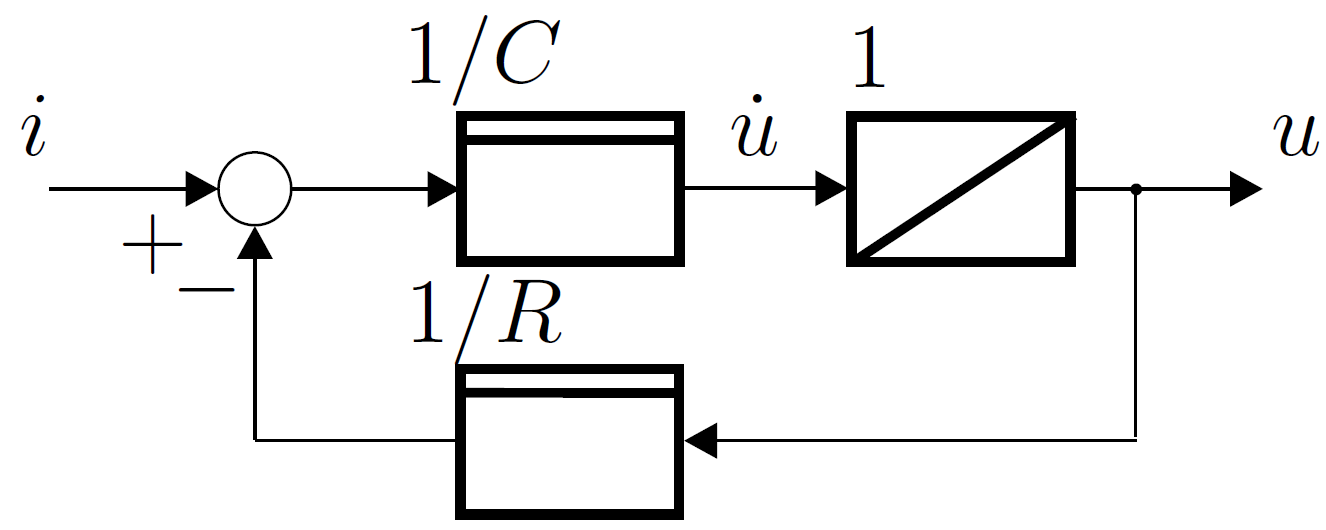
\includegraphics[width=\columnwidth]{images/RegT1_grundglieder/pT1_blockschaltbild}
\end{minipage}
\hfill
\begin{minipage}{0.48\columnwidth}
    $$ \boxed{ \text{Allg: } T \, \dot{y}(t) + y(t) = K \cdot u(t) }  $$
    $$ \boxed{ \text{Bsp: } RC \, \dot{u}(t) + u(t) = R \cdot i(t) }  $$
\end{minipage}

%\columnbreak


\subsection[PT2-Glied]{$\text{PT}_2$-Glied}

Zwei Energiespeicher \textrightarrow\ \textbf{System kann schwingen}

\vspace{-0.1cm}

\begin{minipage}{0.4\columnwidth}
    $$ \boxed{ \text{DGL: } T^2 \cdot  \ddot{y} + 2 \, \zeta \, T \cdot \dot{y} + y = K \cdot u } $$
\end{minipage}
\hfill
\begin{minipage}{0.58\columnwidth}
    $$ \boxed{ y(t) = K \: A \big[ 1 + e^{\sigma t} \big( - \cos(\omega t) + \frac{\sigma}{\omega} \sin(\omega t)  \big)  \big] }  $$
\end{minipage}


\begin{minipage}{0.55\columnwidth}
    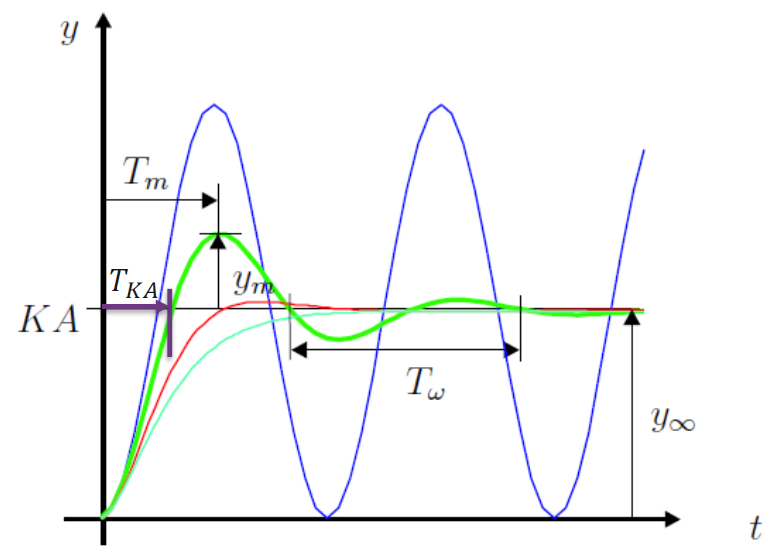
\includegraphics[width=\columnwidth]{images/RegT1_grundglieder/pT2_sprungantwort}
\end{minipage}
\hfill
\begin{minipage}{0.38\columnwidth}
    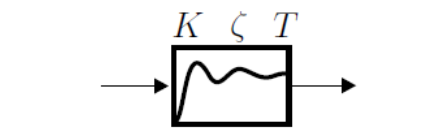
\includegraphics[width=0.75\columnwidth]{images/RegT1_grundglieder/pT2_symbol} 

    \begin{center}
        $ \omega = \omega_n \cdot \sqrt{1 - \zeta^2} $ \\
        $y_m = e^h \cdot y_{\infty}$ \\
    \end{center}
\end{minipage}


\begin{tabular}{c c c}
    $ K = \frac{y_{\infty}}{A}$                                                     & $ h = \ln \big( \frac{y_m}{y_{\infty}} \big)$                                 & $ \omega = \frac{2 \, \pi}{T_{\omega}} = \frac{\pi}{T_m} $ \\

    \rule{0pt}{10pt}$ \sigma = \frac{h \, \omega}{\pi} = - \omega_n \cdot \zeta$    & $ \omega_n = \sqrt{\omega^2 + \sigma^2} = - \frac{\sigma}{\zeta}$             & $ \zeta = - \frac{h}{\sqrt{h^2 + \pi^2}} $ \\

    \rule{0pt}{10pt}$T = \frac{1}{\omega_n}$                                        & $T_{KA} = T_M - \frac{1}{\omega} \arctan \big(  \frac{\omega}{\sigma} \big)$  & $y(T_{KA}) = K \: A$ \\
\end{tabular}

\vspace{0.2cm}
\textrightarrow\ $\zeta = \frac{1}{\sqrt{2}}$ entspricht 5 \% Überschwingen!


\subsection{D-Glied (Idealer Differenzierer)}

\vspace{-0.2cm}

$$ \boxed{  y(t) = K \cdot \frac{\diff u(t)}{\diff t} = K  \cdot \dot{u}(t) } $$

\begin{minipage}{0.25\columnwidth} 
    \begin{center}
        \myul{\textbf{ideal}}
    \end{center}

    \vspace{-0.1cm}

    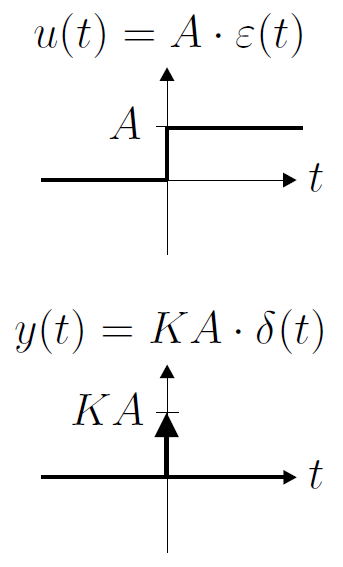
\includegraphics[width=0.65\columnwidth]{images/RegT1_grundglieder/D-glied_ideal}
\end{minipage}
\hfill
\begin{minipage}{0.25\columnwidth}
    \begin{center}
        \myul{\textbf{real}}
    \end{center}

    \vspace{-0.1cm}

    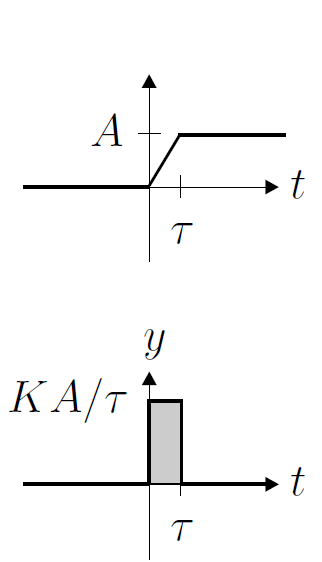
\includegraphics[width=0.6\columnwidth]{images/RegT1_grundglieder/D-glied_real}
\end{minipage}
\hfill
\begin{minipage}{0.25\columnwidth}
    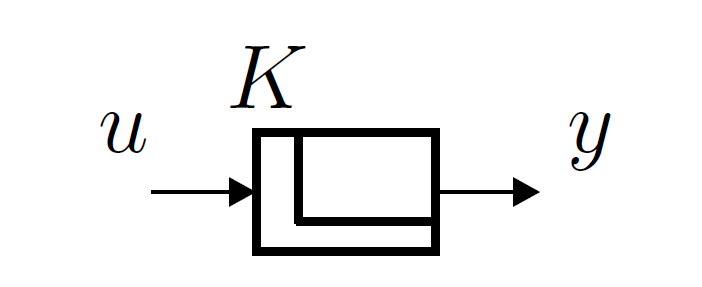
\includegraphics[width=0.9\columnwidth]{images/RegT1_grundglieder/D-glied_symbol}
\end{minipage}


\subsection[DT1-Glied (Realisierbarer Differenzierer)]{$\text{DT}_1$-Glied (Realisierbarer Differenzierer)}

\vspace{-0.1cm}

\begin{minipage}{0.48\columnwidth}  
    $$ \boxed{ w(t) = A \cdot (1 - e^{-\frac{t}{T}}) } $$
\end{minipage}
\hfill
\begin{minipage}{0.48\columnwidth}
    $$ \boxed{ y(t) = \frac{K \cdot A}{T} \,  e^{-\frac{t}{T}} } $$
\end{minipage}

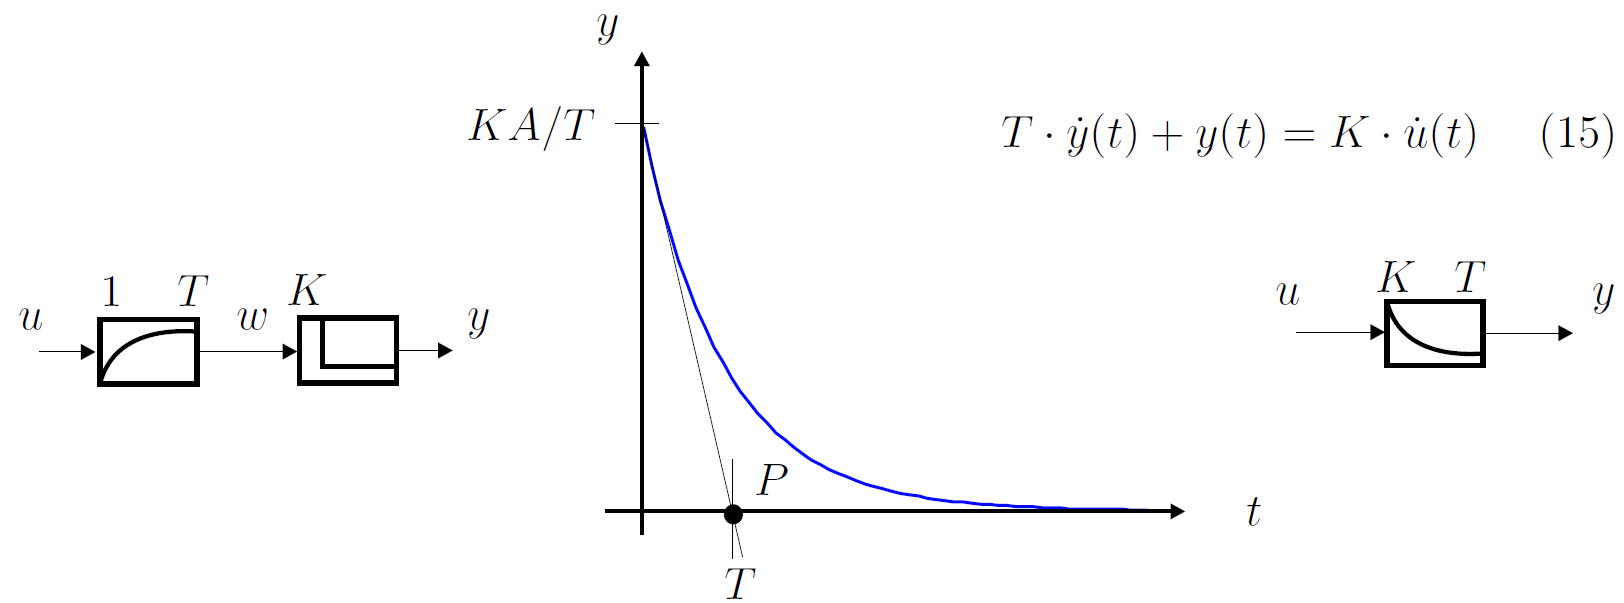
\includegraphics[width=\columnwidth]{images/RegT1_grundglieder/DT1-glied}


\example{Mögliche Realisierungen von $\text{DT}_1$-Gliedern}

\begin{minipage}[t]{0.48\columnwidth}
    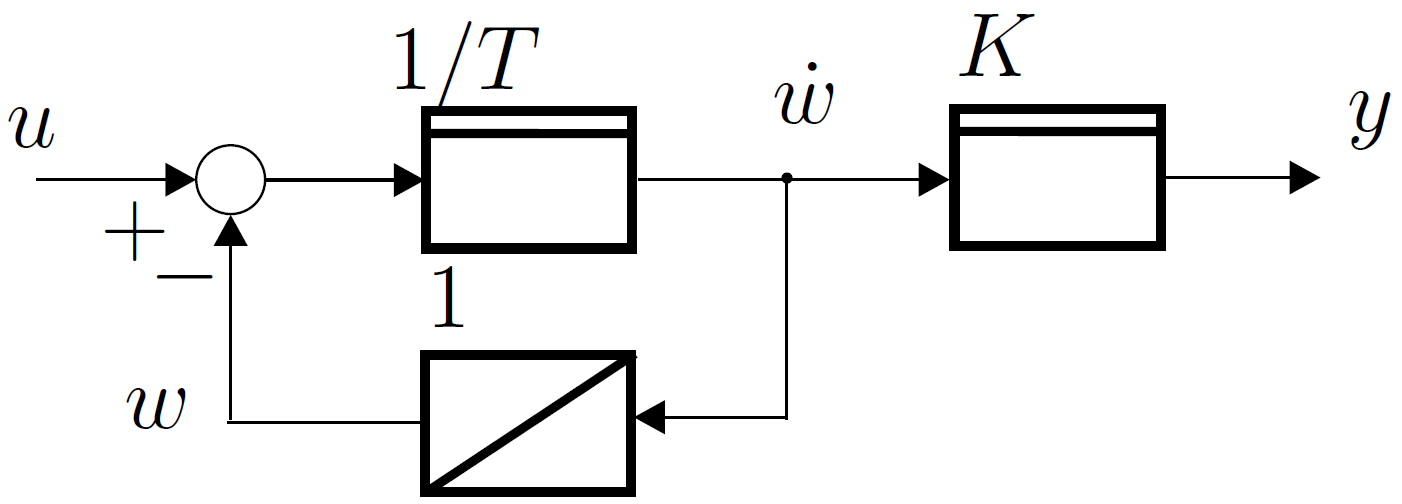
\includegraphics[width=\columnwidth, align=t]{images/RegT1_grundglieder/pT1_blockschaltbild_2}
\end{minipage}
\hfill
\begin{minipage}[t]{0.48\columnwidth}
    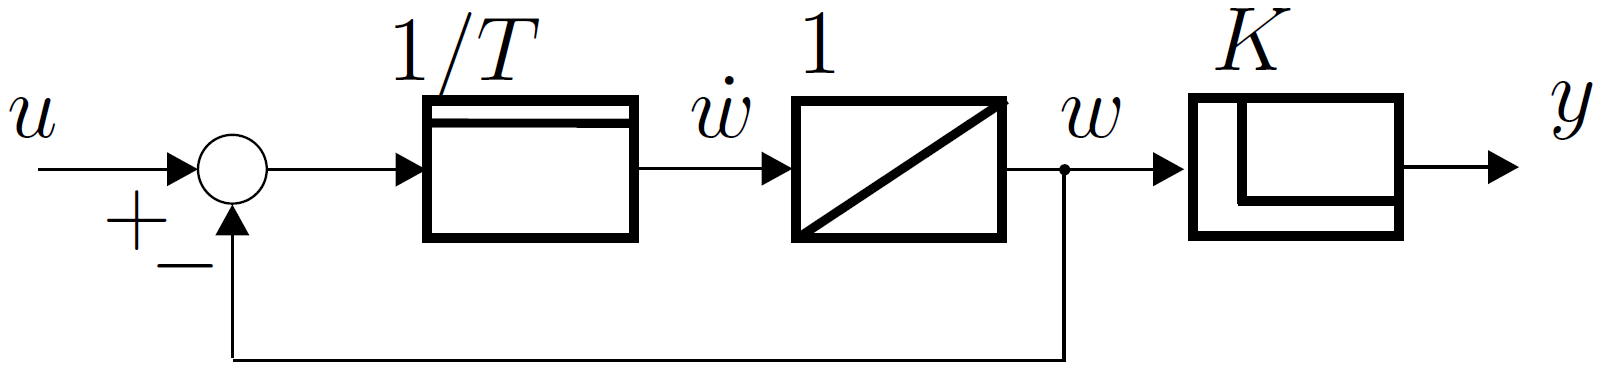
\includegraphics[width=\columnwidth, align=t]{images/RegT1_grundglieder/DT1-glied_blockschaltbild}
\end{minipage}



\subsection{Lead-Glied / Lag-Glied / Lead-Lag-Glied}

Lead-/ Lag-Glieder sind zwei Varianten von $\text{PDT}_1$-Gliedern. 

\begin{tabular}{ll}
    Lead:   & $K_P$ und $K_D$ haben \textbf{gleiches} Vorzeichen \\
    Lag:    & $K_P$ und $K_D$ haben \textbf{unterschiedliches} Vorzeichen \\
\end{tabular}

Lead- und Lag-Glieder können auch als Parallelschaltungen eines P- und eines $\text{PT}_1$-Glieds aufgefasst werden. 
Das Lead-Lag-Glied ist eine Serieschaltung aus Lead- und Lag-Glied.

\vspace{0.2cm}

\begin{minipage}[t]{0.45\columnwidth}
    \begin{center}
        \myul{\textbf{Lead-Glied}}
    \end{center}
    
    \vspace{-0.1cm}

    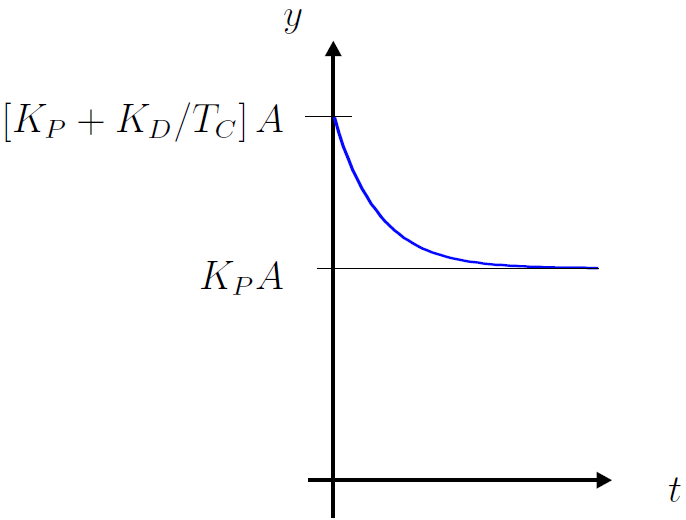
\includegraphics[width=0.9\columnwidth, align=t]{images/RegT1_grundglieder/lead-glied}
\end{minipage}
\hfill
\begin{minipage}[t]{0.45\columnwidth}
    \begin{center}
        \myul{\textbf{Lag-Glied}}
    \end{center}
    
    \vspace{-0.1cm}

    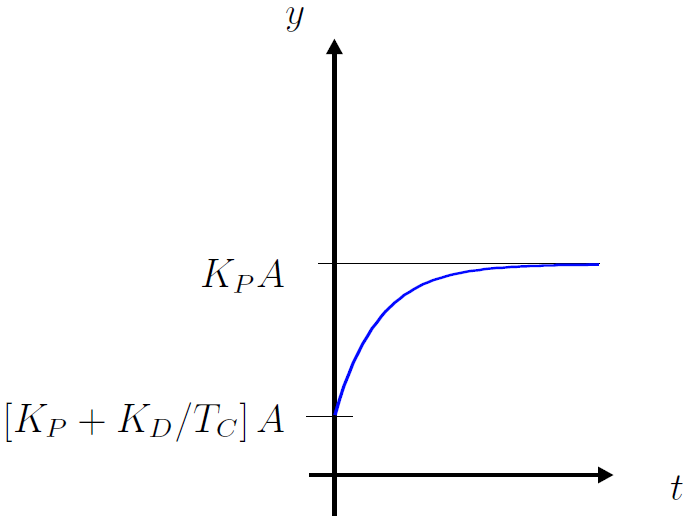
\includegraphics[width=0.9\columnwidth, align=t]{images/RegT1_grundglieder/lag-glied}
\end{minipage}

\section*{Prüfungscheck / Schnellreferenz}

\subsection*{Steuerbarkeit}
\[
Q_S=[B \;\; AB \;\; A^2B \;\; \dots \;\; A^{n-1}B]
\]

Vollständig steuerbar:
\[
\mathrm{rang}(Q_S)=n
\]

Steuerbar:
\[
\det(Q_S)\neq0
\]
(SISO-Fall)

\subsection*{Beobachtbarkeit}
\[
Q_B=
\begin{bmatrix}
C\\
CA\\
CA^2\\
\vdots\\
CA^{n-1}
\end{bmatrix}
\]

Vollständig beobachtbar:
\[
\mathrm{rang}(Q_B)=n
\]

\subsection*{Minimalität}
System minimal
\[
\Longleftrightarrow
\]
steuerbar \textbf{und} beobachtbar.

\subsection*{Zustandsrückführung}
\[
u=-Kx+r
\]

Geschlossener Kreis:
\[
\dot x=(A-BK)x+Br
\]

Pole:
\[
\lambda(A-BK)
\]

Polvorgabe nur möglich falls:
\[
\mathrm{rang}(Q_S)=n
\]

\subsection*{Beobachter}
\[
\dot{\hat x}=A\hat x+Bu+H(y-\hat y)
\]

\[
\hat y=C\hat x
\]

Beobachterpole:
\[
\lambda(A-HC)
\]

\subsection*{Transitionsmatrix}
\[
\Phi(t)=e^{At}
\]

\[
A=\dot{\Phi}(0)
\]

Diagonalform:
\[
e^{\Lambda t}
=
\mathrm{diag}
\left(
e^{\lambda_1 t},
\dots,
e^{\lambda_n t}
\right)
\]

\subsection*{Impulsantwort}
Kontinuierlich:
\[
g(t)=Ce^{At}B+D\delta(t)
\]

Diskret:
\[
g(k)=CA^{k-1}B
\qquad (k\ge 1)
\]

\subsection*{Stabilität}
Zeitkontinuierlich:
\[
\mathrm{Re}(\lambda_i)<0
\]

Zeitdiskret:
\[
|\lambda_i|<1
\]

\subsection*{Trajektorienbilder}
\begin{itemize}
\item $\lambda<0$: Ursprung attraktiv
\item $\lambda>0$: Ursprung abstossend
\item $\lambda=\pm j\omega$: Kreisbewegung
\item Jordanblock: Scherbewegung
\end{itemize}

\subsection*{Prüfungsklassiker}
\begin{itemize}
\item UTF $\leftrightarrow$ ZRD
\item Blockdiagramm $\rightarrow$ ZRD
\item Steuerbarkeit / Beobachtbarkeit
\item Polvorgabe
\item Transitionsmatrix
\item Impulsantwort / Faltung
\item ZOH-Diskretisierung
\item Wurzelortskurve
\end{itemize}

\subsection*{Sofortwissen}

\[
G(s)=C(sI-A)^{-1}B+D
\]

\[
\tilde A=PAP^{-1}
\]

\[
\tilde B=PB
\]

\[
\tilde C=CP^{-1}
\]

Eigenwerte bleiben bei der Ähnlichkeitstransformation unverändert.